\chapter{Setup of data and project}
In this chapter we will discuss the setup of the project.

\section{Getting familiar with the data}
Before the project was set-up the initial task was to gather information for calculating one of the first defined and most basic codon bias index called \hyperlink{function:Fop}{frequency of optimal codons (Fop)}. The optimality of a codon can be estimated by the usage in the given gene, the transcriptome or by accessing the numbers of tRNA genes found in the genome. As we have already the \hyperlink{data:tRNAlist}{data of tRNA genes for the teff genome} available, this was the choice to work with and to import the information for closely related species for mays and millet.

\subsection{read tRNA stats and decide on optimality of a codon}
  \lstinputlisting[language=R, breaklines=true]{codes/readstats.R}
  \lstinputlisting[language=HTML, breaklines=true]{codes/Zmays.stats}    
 
However this code had to be adapted because it is only reading in the tRNA genes with introns. Interestingly, by browsing some of the output data from tRNAscan for other species we discovered some that have a huge amount of the alternative usage of the opal stop codon "UGA" that is messing up with the display of the overview in a hierarchical plot for all the tRNA numbers even when standardized for each tRNA, we can see that some of the species show a much higher total number of tRNAs. 

\begin{figure}[tb] 
\centering 
\includegraphics[width=0.9\columnwidth]{byrow} 
\caption[Heat map for tRNA counts]{Heat map of tRNA gene counts normalized per row in \hyperlink{data:veab}{all species}}
\label{fig:byrow} 
\end{figure}

If we plot the log values of the tRNA gene count and normalize by species (column) then we can see that some species have very low numbers of certain codons that is usually compensated by using another block of codons that are rare in the other kingdoms. We also observe some species that have a high number of tRNAs where the isoaccepter remains unknown (codon 65).


\begin{figure}[tb] 
\centering 
\includegraphics[width=0.9\columnwidth]{logallfa_col} 
\caption[Heat map for log(tRNA counts)]{Heat map of logged(tRNA gene counts) normalized per column in \hyperlink{data:veab}{all species}}
\label{fig:bycol} 
\end{figure}


\section{text chunk - tRNA database}
The tRNA genome numbers for eukariotic, bacterial, archaea and one viral genome was extracted from tRNAscan-SE v.1.3 run statistics of the GtRNAdb 2.0 (available at
\href{http://gtrnadb.ucsc.edu/GtRNAdb2/genomes/}{Genomic tRNA Database 2.0}, http://gtrnadb.ucsc.edu/GtRNAdb2/genomes/). \cite{Chan2016}[Chan PP et al. 2016]

To decide on optimal codons the number of genes for the given anticodon was divided by the maximal number of genes for a anticodon for the same aminoacid to give fraction to optimal codon. The codon was accepted as optimal if this fraction was 1. In a list for every genome with available run statistic data, a frame with aminoacid, codon, number of genes, fraction to optimal codon, fraction to all codons, and the decision if it is a optimal codon was stored for the four superkingdoms seperately.
 
\begin{verbatim}
 The genomes with names containing # or * have to be treated as special 
 cases, as even the browser failed to fetch the files. 
 Therefore # was replaced with %23
\end{verbatim}

However, in those run statistics, from vertebrates especially non-primate mammals, are littered with tRNA-derived repetitive elements with primary sequences very similar to real tRNAs. So they apply a non-unveiled post filter after the tRNAscan-SE on those genomes before depositing the predictions to GtRNAdb. Therefore, and because they were not willing to share the database with the summary statistics, these had to be rebuild from scanning the headers of the fasta files. Therefore the fasta file name had to be scanned in the index.html file and the fasta files were renamed according to the directory name to facilitate automation. 

The statistics is now enhanced by an 65th line containing undefined aminoacid all other anticodons with degenerated base information are counted to the undefined species (as they do in the summary page)

codon ramp (rare codons at the start Tuller et al.) "This “codon ramp” hypothesis should apply primarily in the context of strong translation, but we found that using rare codons at the N terminus increases expression regardless of translation strength." --ANECTODE-- When analysing the moving average of the optionality factor of the codons for the tRNA genes, we don't really detect a codon ramp at the 5' terminus, first, but the first codon was always optimal. No wonder because there is only one codon for Methionine, the start codon. Therefore we should only analyse the aminoacids that have a choice of anti-codons to use.  

For analyzing codon usage in E. teff Gina's validated protein-transcript fasta files were used, however there were two issues in the database: 
first one of the proteins (
Et\_s4372-0.17-1
) was truncated, didn't startet with methionine and was not corresponding to the truncated transcript, secondly the number of transcripts matched the number of proteins, but there was one orphan entry on each side (
Et\_s2692-0.26-1, Et\_s14755-0.7-1
), that had to be filled up with the corresponding entry of the other datafile. 


\subsection{text chunk - Project notes}
The first index to be implemented was the frequency of optimal codons. When the decision on which codons are optimal is made, the calculation of this index is quite basic. The decision can be made by taking the codon usage of the gene alone or the full genome or what we intended to implement first was to make the decision on the availability of tRNAs estimated from the number of tRNA genes that we find in the genome of \textit{E. tef}. For generalization of the function we scanned available information on tRNA gene counts from a public database. However, the retrieved tRNA database turned out to make some problems: \\
Some of the species had a much higher number of tRNA genes, so that a normalization was necessary to get an overview on the used codons. %, anomolous values solutions: standardize data \\
% computed codon usage in tef problems: odd characters in data, mismatch, solution: preprocess data
% sequences in frame: solution: preprocess data
%is implementation of a suffix tree a possibility?

% testing - use the sequences form the original papers and show that you get the same values

The project is based on three pillars, namely the code itself, the testing functions and the documentation, including demonstration scripts.

%start with CAI
% look at implementatino in seqinR-  what is available already in SeqinR? use as much of their stuff as possible but we want to keep the possibility to change base data if you want (tRNA mapping and frequencies)
% look at what the possibilities are and what parts of the exisiting implementation can be used?
% if not , reimplement in such a way that it is more flexible 


\subsection{Plot OCU demo}
\begin{figure}[tb] 
\centering 
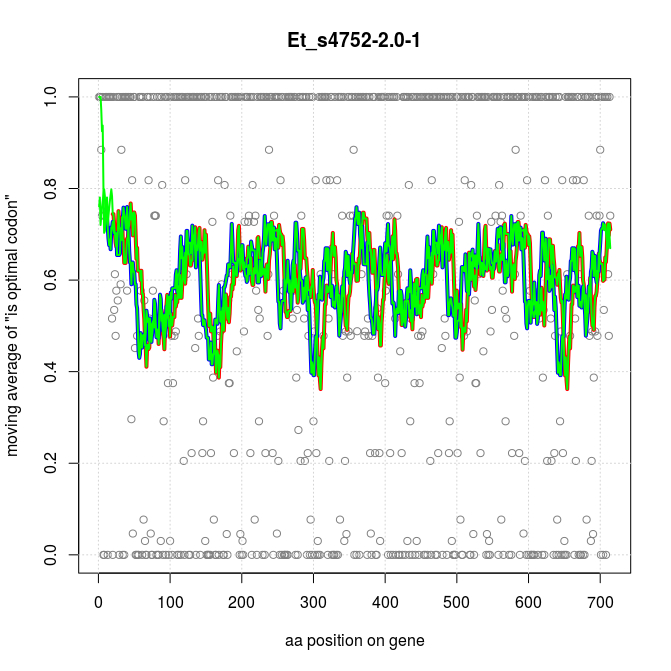
\includegraphics[width=0.9\columnwidth]{fig1_plotOCU} 
\caption[A sample figure from demo plotOCU]{A sample figure (from plot OCU \emph{demo(plotOCU)}, of statanacoseq, got from \url{https://github.com/fredysiegrist/statanacoseq}) shwoing the optimality score of each codon used for coding Similar to Eukaryotic peptide chain release factor subunit 1-3 (eRF1-3) gene of teff.}
\label{fig:plotOCU} 
\end{figure}
